%iffalse
\let\negmedspace\undefined
\let\negthickspace\undefined
\documentclass[journal,12pt,onecolumn]{IEEEtran}
\usepackage{cite}
\usepackage{amsmath,amssymb,amsfonts,amsthm}
\usepackage{algorithmic}
\usepackage{multicol}
\usepackage[latin1]{inputenc}
\usepackage{circuitikz}
\usepackage{tikz}
\usepackage{graphicx}
\usepackage{textcomp}
\usepackage{xcolor}
\usepackage{txfonts}
\usepackage{listings}
\usepackage{enumitem}
\usepackage{mathtools}
\usepackage{gensymb}
\usepackage{comment}
\usepackage[breaklinks=true]{hyperref}
\usepackage{tkz-euclide} 
\usepackage{listings}
\usepackage{gvv} 
\usepackage{tikz}
\usetikzlibrary{shapes,arrows} 

%\def\inputGnumericTable{}                                
\usepackage[latin1]{inputenc}                                
\usepackage{color}                                            
\usepackage{array}                                            
\usepackage{longtable}                                       
\usepackage{calc}                                             
\usepackage{multirow}
\usepackage{amsmath}
\usepackage{pgfplots}
\usepackage{graphicx}
\usepackage{hhline}                                           
\usepackage{ifthen}                                           
\usepackage{lscape}
\usepackage{tabularx}
\usepackage{array}
\usepackage{float}
\newcommand{\rupee}{\text{Rs.}}
\newtheorem{theorem}{Theorem}[section]
\newtheorem{problem}{Problem}
\newtheorem{proposition}{Proposition}[section]
\newtheorem{lemma}{Lemma}[section]
\newtheorem{corollary}[theorem]{Corollary}
\newtheorem{example}{Example}[section]
\newtheorem{definition}[problem]{Definition}
\newcommand{\BEQA}{\begin{eqnarray}}
\newcommand{\EEQA}{\end{eqnarray}}
\newcommand{\define}{\stackrel{\triangle}{=}}
\theoremstyle{remark}


% Marks the beginning of the document
\begin{document}
\bibliographystyle{IEEEtran}
\vspace{3cm}

\title{\textbf{2024-DA-1-13}}
\author{EE24BTECH11052 - RONGALI CHARAN}
\maketitle
\bigskip

\renewcommand{\thefigure}{\theenumi}
\renewcommand{\thetable}{\theenumi}
\setlength{\columnsep}{2.5em}\begin{enumerate}
\item If \textquoteleft{} $\rightarrow$ \textquoteright{} denotes increasing order of intensity, then the meaning of the words
\texttt{[sick $\rightarrow$ infirm $\rightarrow$ moribund]} is analogous to \texttt{[silly $\rightarrow$ \_\_\_\_\_ $\rightarrow$ daft]}.

Which one of the given options is appropriate to fill the blank?

\begin{enumerate}
    \item frown
    \item fawn
    \item vein
    \item vain
\end{enumerate}
\item The 15 parts of the given figure are to be painted such that no two adjacent parts with shared boundaries (excluding corners) have the same color. The minimum number of colors required is:
	\begin{center}
		

\begin{circuitikz}[scale=0.4, transform shape] % Small size with scale 0.4
    \tikzstyle{every node}=[font=\LARGE]

    \draw  (-7.5,19.75) ellipse (7.75cm and 6cm);
    \draw  (-10.5,23.75) rectangle (-4.5,15.25); % Rectangle without text
    \draw  (-7.5,20) circle (2cm);
    \draw [short] (-10.5,23.75) -- (-8.75,21.5);
    \draw [short] (-6.25,21.5) -- (-4.5,23.75);
    \draw [short] (-10.5,15.25) -- (-8.5,15.25);
    \draw [short] (-10.5,15.25) -- (-8.75,18.5);
    \draw [short] (-6.5,18.25) -- (-4.5,15.25);
    \draw [short] (-7.5,20) -- (-7.5,22);
    \draw [short] (-7.5,20) -- (-9.25,19);
    \draw [short] (-7.5,20) -- (-5.75,19);
    \draw [short] (-10.5,23.75) -- (-9,25.75);
    \draw [short] (-10.5,23.75) -- (-13.5,23.5);
    \draw [short] (-4.5,23.75) -- (-5,25.5);
    \draw [short] (-4.5,23.75) -- (-1,23);
    \draw [short] (-4.5,15.25) -- (-1,16.75);
    \draw [short] (-4.5,15.25) -- (-5.25,14);
    \draw [short] (-10.5,15.25) -- (-13.75,16.25);
    \draw [short] (-10.5,15.25) -- (-9.75,14);
\end{circuitikz}



	\end{center}

\begin{enumerate}
    \item 4
    \item 3
    \item 5
    \item 6
\end{enumerate}
\item How many 4-digit positive integers divisible by 3 can be formed using only the digits \{1, 3, 4, 6, 7\}, such that no digit appears more than once in a number?
\begin{enumerate}
    \item 24
    \item 42
    \item 78
    \item 12
\end{enumerate}
\item The sum of the following infinite series is
$$2 + \frac{1}{2} + \frac{1}{3} + \frac{1}{4} + \frac{1}{8} + \frac{1}{9} + \frac{1}{16} + \frac{1}{27} + \dots $$
\begin{enumerate}
     \item $\frac{11}{3}$
     \item $\frac{7}{2}$
     \item $\frac{13}{4}$
     \item $\frac{9}{2}$
\end{enumerate}
\item In an election, the share of valid votes received by the four candidates A, B, C, and D is represented by the pie chart shown. The total number of votes cast in the election were 1,15,000, out of which 5,000 were invalid.
\begin{center}
	\begin{circuitikz}[scale=0.6]
\tikzstyle{every node}=[font=\LARGE]
\draw  (-9,21.75) circle (3.5cm);
\draw [short] (-9,21.75) -- (-9,25.25);
\draw [short] (-9,21.75) -- (-6.5,19.25);
\draw [short] (-9,21.75) -- (-11.75,19.5);
\draw [short] (-9,21.75) -- (-12,23.5);
\node [font=\large] at (-7.25,23.25) {A};
\node [font=\large] at (-9,20.25) {B};
\node [font=\large] at (-11.5,22.25) {C};
\node [font=\large] at (-10.25,24.25) {D};
\node [font=\large] at (-7.25,22) {40\%};
\node [font=\large] at (-9,19.25) {25\%};
\node [font=\large] at (-11.25,21.25) {20\%};
\node [font=\large] at (-10,23.5) {15\%};
\end{circuitikz}




\end{center}
Based on the data provided, the total number of valid votes received by the candidates B and C is:

\begin{enumerate}
    \item 45,000
    \item 49,500
    \item 51,750
    \item 54,000
\end{enumerate}
\item Thousands of years ago, some people began dairy farming. This coincided with a number of mutations in a particular gene that resulted in these people developing the ability to digest dairy milk.//


Based on the given passage, which of the following can be inferred?
\begin{enumerate}
    \item All human beings can digest dairy milk.
    \item No human being can digest dairy milk.
    \item Digestion of dairy milk is essential for human beings.
    \item In human beings, digestion of dairy milk resulted from a mutated gene.
\end{enumerate}
\item The probability of a boy or a girl being born is $ \frac{1}{2} $. For a family having only three children, what is the probability of having two girls and one boy?
\begin{enumerate}
    \item $ \frac{3}{8} $
    \item $ \frac{1}{8} $
    \item $ \frac{1}{4} $
    \item $ \frac{1}{2} $
\end{enumerate}
\item Person 1 and Person 2 invest in three mutual funds A, B, and C. The amounts they invest in each of these mutual funds are given in the table.\\
	\begin{table}[h!]
\centering
\begin{tabular}{|c|c|c|c|}
\hline
                & \textbf{Mutual fund A} & \textbf{Mutual fund B} & \textbf{Mutual fund C} \\ \hline
\textbf{Person 1} & \(\rupee 10,000\)          & \(\rupee 20,000\)          & \(\rupee 20,000\)          \\ \hline
\textbf{Person 2} & \(\rupee 20,000\)          & \(\rupee 15,000\)          & \(\rupee 15,000\)          \\ \hline
\end{tabular}
\end{table}
\\
At the end of one year, the total amount that Person 1 gets is \rupee500 more than Person 2. The annual rate of return for the mutual funds B and C is 15\% each. What is the annual rate of return for the mutual fund A?

\begin{enumerate}
    \item $7.5\%$
    \item $10\%$
    \item $15\%$
    \item $20\%$
\end{enumerate}
\item Three different views of a dice are shown in the figure below.\\
\noindent % To remove indentation for the first figure
\begin{minipage}{0.33\textwidth}
    \centering
    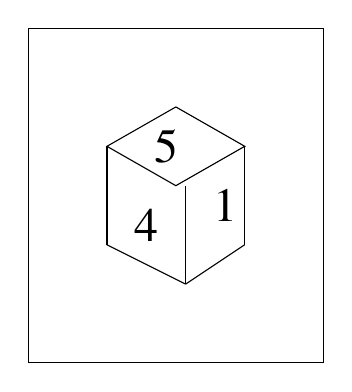
\begin{tikzpicture}
\tikzstyle{every node}=[font=\huge]
\draw[fill={rgb,255:red,255; green,255; blue,255}] (-16.5,24) rectangle (-12.75,19.75);
\draw  (-15.5,22.5) -- (-14.625,22) -- (-13.75,22.5) -- (-14.625,23) -- cycle;
\draw [short] (-15.5,22.5) -- (-15.5,21.25);
\draw [short] (-13.75,22.5) -- (-13.75,21.25);
\draw [short] (-15.5,21.25) -- (-14.5,20.75);
\draw [short] (-14.5,20.75) -- (-13.75,21.25);
\draw [short] (-14.5,20.75) -- (-14.5,22);
\node [font=\LARGE] at (-14.75,22.5) {5};
\node [font=\LARGE] at (-15,21.5) {4};
\node [font=\LARGE] at (-14,21.75) {1};
\end{tikzpicture}

  % Include the first figure code
\end{minipage}%
\begin{minipage}{0.33\textwidth}
    \centering
    
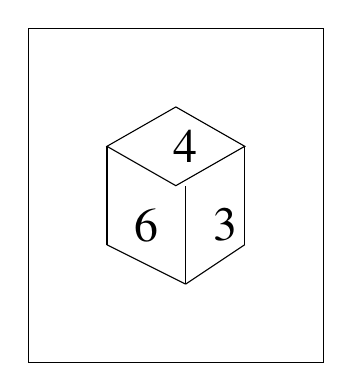
\begin{tikzpicture}
\tikzstyle{every node}=[font=\LARGE]
\draw[fill={rgb,255:red,255; green,255; blue,255}] (-16.5,24) rectangle (-12.75,19.75);
\draw  (-15.5,22.5) -- (-14.625,22) -- (-13.75,22.5) -- (-14.625,23) -- cycle;
\draw [short] (-15.5,22.5) -- (-15.5,21.25);
\draw [short] (-13.75,22.5) -- (-13.75,21.25);
\draw [short] (-15.5,21.25) -- (-14.5,20.75);
\draw [short] (-14.5,20.75) -- (-13.75,21.25);
\draw [short] (-14.5,20.75) -- (-14.5,22);
\node [font=\LARGE] at (-14.5,22.5) {4};
\node [font=\LARGE] at (-15,21.5) {6};
\node [font=\LARGE] at (-14,21.5) {3};
\end{tikzpicture}


  % Include the second figure code
\end{minipage}%
\begin{minipage}{0.33\textwidth}
    \centering
    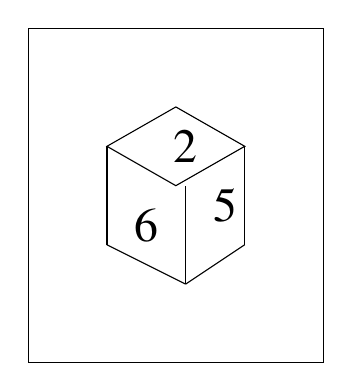
\begin{tikzpicture}
\tikzstyle{every node}=[font=\LARGE]
\draw[fill={rgb,255:red,255; green,255; blue,255}] (-16.5,24) rectangle (-12.75,19.75);
\draw  (-15.5,22.5) -- (-14.625,22) -- (-13.75,22.5) -- (-14.625,23) -- cycle;
\draw [short] (-15.5,22.5) -- (-15.5,21.25);
\draw [short] (-13.75,22.5) -- (-13.75,21.25);
\draw [short] (-15.5,21.25) -- (-14.5,20.75);
\draw [short] (-14.5,20.75) -- (-13.75,21.25);
\draw [short] (-14.5,20.75) -- (-14.5,22);
\node [font=\LARGE] at (-15,21.5) {6};
\node [font=\LARGE] at (-14.5,22.5) {2};
\node [font=\LARGE] at (-14,21.75) {5};
\end{tikzpicture}

  % Include the third figure code
\end{minipage}\\
The piece of paper that can be folded to make this dice is
\begin{enumerate}
	\item 
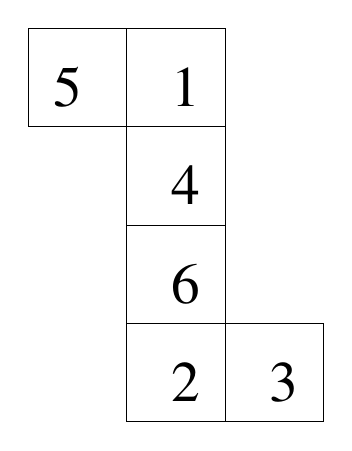
\begin{tikzpicture}
\tikzstyle{every node}=[font=\huge]
\draw  (-21.25,24.75) rectangle (-20,23.5);
\draw  (-20,24.75) rectangle (-18.75,23.5);
\draw  (-20,23.5) rectangle (-18.75,22.25);
\draw  (-20,22.25) rectangle (-18.75,21);
\draw  (-20,21) rectangle (-18.75,19.75);
\draw  (-18.75,21) rectangle (-17.5,19.75);
\node [font=\huge] at (-20.75,24) {5};
\node [font=\huge] at (-19.25,24) {1};
\node [font=\huge] at (-19.25,22.75) {4};
\node [font=\huge] at (-19.25,21.5) {6};
\node [font=\huge] at (-19.25,20.25) {2};
\node [font=\huge] at (-18,20.25) {3};
\end{tikzpicture}


	\item \usetikzlibrary{decorations.markings, arrows, arrows.meta}

\tikzset{
    midar/.style={
        very thick,
        decoration={
            markings,
            mark=at position 0.55 with {\arrow{latex}}, % Arrow only at the midpoint
        },
        postaction=decorate,
    },
}

\begin{tikzpicture}[thick]
    % Shortened Axes
    \draw[-{Latex}] (0,0) -- (0,3.5) node[above] {$T$};
    \draw[-{Latex}] (0,0) -- (4.5,0) node[right] {$S$};

    % Points and labels
    \node at (1,2.5) [above left] {3};
    \node at (2.5,2.5) [below left] {1};
    \node at (3,1) [below right] {2};

    % Straight line from point 3 to point 1
    \draw[midar] (1,2.5) -- (2.5,2.5);

    % Hyperbolic curve from 3 to 1
    \draw[midar] plot[domain=2.5:4, samples=100] (\x, {6.25/\x});

    % Additional hyperbolic curve with specified domain
    \draw[midar] plot[domain=4:1, samples=100] (\x, {2.5/\x^0.34});
\end{tikzpicture}


	\item 
\usetikzlibrary{decorations.markings, arrows.meta}


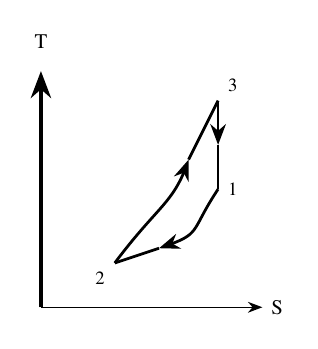
\begin{tikzpicture}[thick, scale=0.75, every node/.style={scale=0.75}]
    % Arrows and lines
    \draw [line width=0.5pt, ->, >=Stealth] (7.5,9.75) -- (11.25,9.75);
    \draw [line width=1.5pt, ->, >=Stealth] (7.5,9.75) -- (7.5,13.75);
    \draw [line width=1pt, ->, >=Stealth] (10.5,13.25) -- (10.5,12.5);
    \draw [line width=1pt, short] (10.5,12.5) -- (10.5,11.75);
    \draw [line width=1pt, ->, >=Stealth] (10.5,11.75) .. controls (10,11) and (10.25,11) .. (9.5,10.75);
    \draw [line width=1pt, short] (9.5,10.75) -- (8.75,10.5);
    \draw [line width=1pt, ->, >=Stealth] (8.75,10.5) .. controls (9.5,11.5) and (9.75,11.5) .. (10,12.25);
    \draw [line width=1pt, short] (10,12.25) -- (10.5,13.25);

    % Node Labels
    \node [font=\small] at (10.75,13.5) {3};
    \node [font=\small] at (10.75,11.75) {1};
    \node [font=\small] at (8.5,10.25) {2};
    \node [font=\normalsize] at (7.5,14.25) {T};
    \node [font=\normalsize] at (11.5,9.75) {S};
\end{tikzpicture}



	\item 
\usetikzlibrary{decorations.markings, arrows.meta}

\tikzset{
    midar/.style={
        very thick,
        decoration={
            markings,
            mark=at position 0.5 with {\arrow{Latex}}, % Arrow at the midpoint
        },
        postaction=decorate,
    },
}

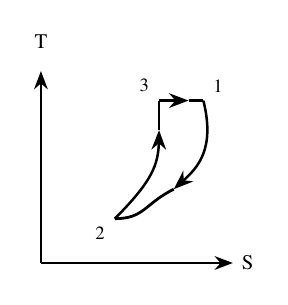
\begin{tikzpicture}[thick, scale=0.75, every node/.style={scale=0.75}]
    % Arrows and lines
    \draw [->, >=Stealth] (7.5,13.5) -- (7.5,16.75);
    \draw [->, >=Stealth] (7.5,13.5) -- (10.75,13.5);
    \draw [line width=0.9pt, ->, >=Stealth] (9.5,16.25) -- (10,16.25);
    \draw [line width=0.9pt, short] (10,16.25) -- (10.25,16.25);
    \draw [line width=0.9pt, ->, >=Stealth] (10.25,16.25) .. controls (10.5,15.25) and (10,15) .. (9.75,14.75) ;
    \draw [line width=1pt, short] (9.75,14.75) .. controls (9.25,14.5) and (9.25,14.25) .. (8.75,14.25);
    \draw [line width=0.9pt, ->, >=Stealth] (8.75,14.25) .. controls (9.5,15) and (9.5,15.25) .. (9.5,15.75) ;
    \draw [line width=0.9pt, short] (9.5,15.75) -- (9.5,16.25);

    % Node Labels
    \node [font=\small] at (10.5,16.5) {1};
    \node [font=\small] at (8.5,14) {2};
    \node [font=\small] at (9.25,16.5) {3};
    \node [font=\normalsize] at (7.5,17.25) {T};
    \node [font=\normalsize] at (11,13.5) {S};
\end{tikzpicture}


	\end{enumerate}
\item Visualize two identical right circular cones such that one is inverted over the other and they share a common circular base. If a cutting plane passes through the vertices of the assembled cones, what shape does the outer boundary of the resulting cross-section make?
\begin{enumerate}
    \item A rhombus
    \item A triangle
    \item An ellipse
    \item A hexagon
\end{enumerate}
\item Consider the following statements:
\begin{itemize}
	\item (i) The mean and variance of a Poisson random variable are equal.
	\item (ii) For a standard normal random variable, the mean is zero and the variance is one.
\end{itemize}
Which ONE of the following options is correct?

\begin{enumerate}
    \item  Both (i) and (ii) are true
    \item  (i) is true and (ii) is false
    \item  (ii) is true and (i) is false
    \item  Both (i) and (ii) are false
\end{enumerate}
\item Three fair coins are tossed independently. T is the event that two or more tosses result in heads. S is the event that two or more tosses result in tails. What is the probability of the event $T \cap S$?

\begin{enumerate}
    \item  0
    \item  0.5
    \item  0.25
    \item  1
\end{enumerate}
\item Consider the matrix $\vec{M} &=  \myvec{2 & -1\\3 & 1}$\\
Which ONE of the following statements is TRUE?

\begin{enumerate}
    \item  The eigenvalues of $\vec{M}$ are non-negative and real.
    \item  The eigenvalues of $\vec{M}$ are complex conjugate pairs.
    \item  One eigenvalue of $\vec{M}$ is positive and real, and another eigenvalue of $\vec{M}$ is zero.
    \item  One eigenvalue of $\vec{M}$ is non-negative and real, and another eigenvalue of $\vec{M}$ is negative and real.
\end{enumerate}















\end{enumerate}



\end{document}
